\documentclass{scrartcl}
\usepackage[a4paper,left=1in,right=1in,top=1.2in,bottom=1in]{geometry}
\usepackage{siunitx}
\usepackage{graphicx}
\usepackage{mathtools}
\setkomafont{disposition}{\normalfont\bfseries}
\newcommand*\diff{\mathop{}\!\mathrm{d}}
\newcommand*\Diff[1]{\mathop{}\!\mathrm{d^#1}}
\newcommand*\colvec[3][]{
    \begin{pmatrix}\ifx\relax#1\relax\else#1\\\fi#2\\#3\end{pmatrix}
}

%title
\title{Exercise 02:\\State space analysis}
\subtitle{Theoretical Neuroscience II}
\author{Johannes G\"atjen \and Lorena Morton}

%use these for structure/overview
\newcommand\Question{%
  \textbf{Question:}%
}
\newcommand\Answer{%
  \textbf{Answer:}%
}

\begin{document}
\maketitle

\section{Task A}

We investigate a linear recurrent network with 2 populations. The time-development is given by the equation

\begin{align*}
\frac{\diff \mathbf{v}}{\diff t} = \mathbf{A} \cdot \mathbf{v} + \mathbf{b} \qquad \text{ with } \qquad \mathbf{A} =  \left( \begin{array}{cc}
-2 & 3 \\
-3 & 2 \end{array} \right).
\end{align*}

We determine the input vector $\mathbf{b}$ such that the steady state of the network is at

\begin{align*}
\mathbf{v}_{ss} = \colvec{10}{10} \qquad \text{ by solving the equation } \qquad \mathbf{A} \cdot \mathbf{v}_{ss} + \mathbf{b} = 0. \\
\shortintertext{Substituting our values we obtain:}
\left( \begin{array}{cc}
-2 & 3 \\
-3 & 2 \end{array} \right) \cdot \colvec{10}{10} + \mathbf{b} &= \colvec{10}{-10} + \mathbf{b} = 0 \\
\Leftrightarrow  \mathbf{b} &= \colvec{-10}{10} \\
\shortintertext{With this we get the full dynamic equation:}
\colvec{\frac{\diff v_1}{\diff t}}{\frac{\diff v_2}{\diff t}} =  \left( \begin{array}{cc}
-2 & 3 \\
-3 & 2 \end{array} \right) \cdot \colvec{v_1}{v_2} + \colvec{-10}{10} \\
\shortintertext{And we get two line equations when we set the gradient for both populations to zero:}
\text{$v_1$-isocline:} & -2 v_1 + 3 v_2 - 10 = 0 \\
\Leftrightarrow & v_2 = \frac{2}{3} v_1 + \frac{10}{3} \\
\text{$v_2$-isocline:} & -3 v_1 + 2 v_2 + 10 = 0 \\
\Leftrightarrow & v_2 = \frac{3}{2} v_1 - 5 \\
\shortintertext{Get the intersection point, by solving the system of linear equations for $v_1$ and $v_2$.}
& \frac{2}{3} v_1 + \frac{10}{3} = \frac{3}{2} v_1 - 5 \\
\Leftrightarrow & v_1 = 10 \\
\shortintertext{Replace the value in one of the original equations.}
v_2 = \frac{3 \cdot 10}{2} - 5 = 10 \\
\shortintertext{And we have confirmed that the steady state is}
\mathbf{v}_{ss} = \colvec{10}{10}.
\end{align*}

\section{Task B}

We obtain the eigenvalues of the connectivity matrix by solving the characteristic equation.
\begin{align*}
&(-2 - \lambda) \cdot (2 - \lambda) + 9 = 0 \\
\Leftrightarrow & -4 + 2\lambda - 2\lambda + \lambda^2 + 9 = 0 \\
\Leftrightarrow & \lambda^2 = -5 \\
\Leftrightarrow & \lambda_1 = i\sqrt{5} \qquad \lambda_2 = -i\sqrt{5} 
\end{align*}
Because $Im(\lambda_1) = - Im(\lambda_2)$ we expect a spiraling behavior from the dynamical system, and because $Re(\lambda_1) = Re(\lambda_2) = 0$ it is neutrally stable.

\begin{figure}
\centering
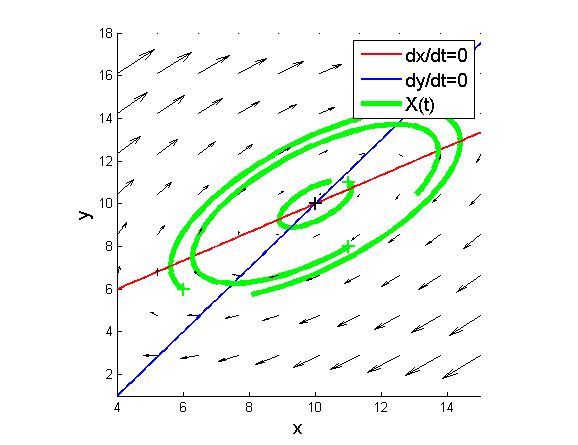
\includegraphics[trim = {1.3cm 0 0.5cm 0.2cm}, width=0.7\textwidth, clip]{../pics/traj}
\caption{Three trajectories of the population activity in the state space for the linear recurrent network.}
\label{label}
\end{figure}

\section{Task C}

As $\kappa$ increases, the frequency of the oscillations do not change, but the steady state value for the amplitude of the oscillations gets smaller, such that the trajectory is damped more strongly. The steady state also appears to change from neutrally stable to stable with higher $\kappa$.

\begin{figure}
\centering
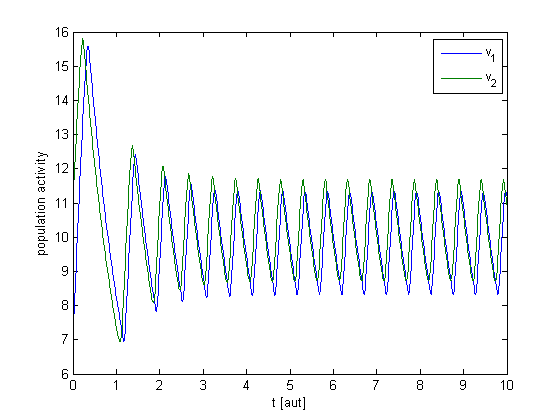
\includegraphics[trim = {0.8cm 0 0.5cm 0.2cm}, width=0.7\textwidth, clip]{../pics/nonlin}
\caption{The evolution of the activity of the two populations over time for the non-linear recurrent network, with $\kappa = 2$.}
\label{label}
\end{figure}

\begin{figure}
\centering
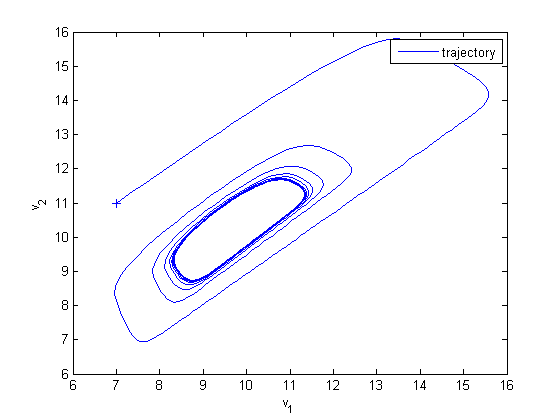
\includegraphics[trim = {0.8cm 0 0.5cm 0.2cm}, width=0.7\textwidth, clip]{../pics/nonlintraj}
\caption{The trajectory of the population activity in the state space for the non-linear recurrent network, with initial condition at $(7, 11)$.}
\label{label}
\end{figure}

%\operatorname{\mathbf{v}}(t) = 

%include picture
%\begin{figure}
%\centering
%\includegraphics[trim = {1.3cm 0 2cm 0.9cm}, width=\textwidth, clip]{../pics/picname}
%\caption{caption text}
%\label{label}
%\end{figure}
\end{document}